\chapter{Introduzione}
%buon divertimento, evviva i plasmi.

All'interno di questo corso affronteremo un'introduzione alla fisica dei plasmi, facendo principalmente riferimento a testi come \emph{'Fisica dei plasmi'} di G.Pucella e S.Segre, \emph{'Principles of plasma physics'} di N.A.Krall e A.W.Trivelpiece, \emph{'Plasma physics and fusion energy'} di J.Freidberg.

Vedremo che la trattazione è spesso approssimata, talvolta ignorando completamente alcuni fenomeni poco rilevanti al fine di presentare un'introduzione. 

La descrizione del plasma per molti versi ricalca quella di un fluido ma con grandi differenze a causa delle forze elettromagnetiche in gioco e le minori collisioni.
Mentre i fluidi, pur avendo grosse difficoltà analitiche, hanno un’unica descrizione fisica a tutte le scale, i plasmi presentano tre regimi distinti in cui la fisica è diversa, vi saranno diverse approssimazioni e set di equazioni:

\begin{itemize}
	\item \textbf{regime fluido}: In cui il plasma viene trattato come un continuo, quando le variazioni spaziali e temporali sono molto più lente delle scale cinetiche. Potremo costruire una descrizione a due fluidi mettendo assieme \emph{conservazione della massa}, \emph{equazione del moto}, \emph{conservazione dell'energia}, \emph{equazione di stato} per ciascuna specie (ioni ed elettroni). Questa descrizione può portare poi ad una descrizione ad un fluido comunemente chiamata \textbf{magnetoidrodinamica} (MHD);
	\item \textbf{regime cinetico}: Quando le scale del fenomeno sono paragonabili a quelle caratteristiche del sistema come il raggio di Larmor $r_L$, la lunghezza di Debye $\lambda_D$ o il libero cammino medio $\lambda_{mfp}$, qui saremo tenuti a descrivere il plasma come un sistema di particelle collisionless;
	\item \textbf{regime dissipativo}: È il regime in cui le piccole resistenze, viscosità, collisionalità non trascurabile, o le regioni sottili diventano importanti.
\end{itemize}
\noindent Tutti i regimi presentano forti non linearità; sotto le non linearità si celano modi lineari, ma questi
interagiscono tra loro creando un comportamento complesso.



\subsection{Cosa è un plasma?}  
%\begin{multicols}{2}
	Il plasma è uno stato della materia simile ad un gas ma completamente ionizzato, la sua composizione dipende dal problema fisico che stiamo affrontando, ma in generale è un sistema di cariche slegate con le seguenti caratteristiche:
	\begin{itemize}
		\item \underline{Globalmente neutro}, $n_e \approx n_i$;
		\item \underline{Dominato dalle forze elettromagnetiche}: Le particelle sono abbastanza lontane (o $k_BT$ è abbastanza grande) da avere \[U\ll k_BT\]
		\item \underline{Collisioni rare} (o poco significative): Per questo nei plasmi "non c'è una termodinamica" ma l'energia viene trasferita su scale sempre più piccole senza dissipazione di energia in calore,  per questo può anche succedere che l'energia diluita possa anche ripresentarsi sotto forma di fenomeno a grande scala.
		\item \underline{Comportamento collettivo}:  Le particelle interagiscono con la distribuzione di carica e le correnti di tutto il sistema contemporaneamente.
	\end{itemize}
	
	\begin{figure}[H]
		\centering
		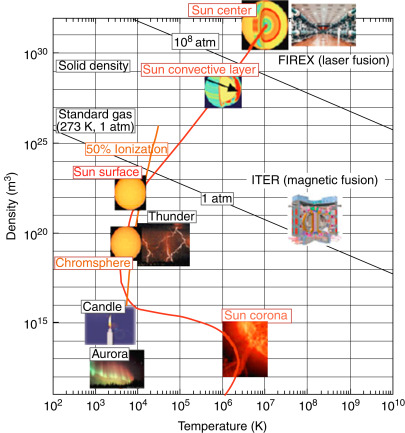
\includegraphics[width=8cm]{immagini/T-rho.jpg}
		\caption{densità e temperature tipiche di alcune diverse manifestazioni dello stato di plasma}
		\label{fig:n-T}
	\end{figure}
%\end{multicols}

Dato che il plasma è relativamente rarefatto, la distanza media tra le cariche è molto maggiore della scala tipica delle interazioni forti ($\lambda_{DB}=\frac{\hbar}{p}\sim10^{-8}$ cm, lunghezza di De~Broglie), $d>>\lambda_{DB}$, per cui non contano gli effetti quantistici, ma prevarranno le forze elettromagnetiche (auto-generate o esterne).

Le collisioni sono estremamente rare e le distanze fra le particelle $r_n$ sono molto maggiori della distanza di minimo approccio $r_0$, , definita da:
\[
\frac{e^2 / r_0}{T} \sim 1
\]. Ciò vuol dire che considerate la \underline{frequenza della dinamica del sistema} $\omega_D$ e la \underline{frequenza collisionale} $\nu_c$:

\[
\text{Per i plasmi: } \frac{\nu_c}{\omega} \rightarrow 0 \quad\quad
\text{Per i gas: } \frac{\nu_c}{\omega} \rightarrow \infty
\]

Il sistema è dominato dalle forze elettromagnetiche: le cariche e il loro moto generano campi elettrici e magnetici, inoltre possono essere presenti campi esterni (elettrici, magnetici o elettromagnetici). 

Si tratta di un sistema N-body, e come nella meccanica statistica è necessario passare a un modello continuo. In fluidodinamica ciò funziona bene; per i plasmi vedremo che la questione è più complessa.


Le equazioni che otterremo sono le equazioni del moto  e l'equazione di continuità, come tipicamente in fluidodinamica. il problema è che in fluidodinamica si può chiudere il sistema con la termodinamica, ma in fisica dei plasmi la termodinamica non ci aiuta molto e bisogna "tirare fuori dal cappello" la chiusura che dobbiamo provare a inventare a seconda della situazione fisica.
